% ============================================================================
% MOCK naskah IEEE Access untuk meninjau tata letak.
% Judul bagian, keterangan gambar/tabel, dan struktur = rancangan draf_struktur.tex (revisi 1).
% Isi teks = lorem ipsum; gambar = sketsa tiruan; angka tabel = isian contoh.
% Kompilasi: pdflatex mock_paper && pdflatex mock_paper   (MiKTeX)
% ============================================================================
% ieeeaccess.cls mendefinisikan ulang primitif \year, yang dipakai pgf saat dimuat.
% Primitifnya disimpan di sini dan dipulihkan sementara saat TikZ dimuat.
\let\primitiveyear\year
\documentclass{ieeeaccess}
\let\accessyear\year
\let\year\primitiveyear
\usepackage{tikz}
\usepackage{pgfplots}
\let\year\accessyear
% pgf menimpa \pdfpageresources; ruang warna spot templat (PANTONE 3015 C, untuk label
% "FIGURE n." dan "TABLE n.") didaftarkan ulang lewat daftar sumber daya milik pgf.
\makeatletter
\expandafter\pgfutil@addpdfresource@colorspaces\expandafter{\the\PANTONE}
\makeatother
\usepackage{cite}
\usepackage{amsmath,amssymb,amsfonts}
\usepackage{algorithm}
\usepackage{algorithmic}
\usepackage{graphicx}
\usepackage{textcomp}
\usepackage{xcolor}
\usepackage{booktabs}
\usepackage{array}
\usepackage{tabularx}
\usepackage{lipsum}
\usetikzlibrary{arrows.meta,positioning,fit,calc,shapes.geometric}
\usepgfplotslibrary{groupplots}
\pgfplotsset{compat=1.16}

\def\BibTeX{{\rm B\kern-.05em{\sc i\kern-.025em b}\kern-.08em
    T\kern-.1667em\lower.7ex\hbox{E}\kern-.125emX}}

\definecolor{cai}{RGB}{226,135,30}
\definecolor{cdet}{RGB}{40,100,170}
\definecolor{chum}{RGB}{40,140,80}
\definecolor{cgr}{RGB}{150,150,150}
\definecolor{cred}{RGB}{200,50,50}
\definecolor{cpur}{RGB}{130,60,160}
\tikzset{
  b/.style={draw, rounded corners=2pt, align=center, font=\scriptsize, minimum height=0.75cm, inner sep=2pt},
  bai/.style={b, fill=cai!18, draw=cai},
  bdet/.style={b, fill=cdet!12, draw=cdet},
  bhum/.style={b, fill=chum!15, draw=chum},
  bsrc/.style={b, fill=white, draw=cgr},
  ar/.style={-{Stealth[length=1.6mm]}, semithick},
  mock/.style={font=\tiny\itshape, text=cgr}
}
\newcolumntype{L}{>{\raggedright\arraybackslash}X}
\newcolumntype{P}[1]{>{\raggedright\arraybackslash}p{#1}}
\newcolumntype{C}{>{\centering\arraybackslash}X}
\newtheorem{definition}{Definition}
% Float "Listing" (paket float sudah dimuat oleh algorithm.sty)
\newfloat{listing}{tbp}{lol}
\floatname{listing}{Listing}
\newcommand{\xx}{\textcolor{cgr}{x.xx}}
\newcommand{\nn}{\textcolor{cgr}{n/N}}

\begin{document}
\history{Date of publication xxxx 00, 0000, date of current version xxxx 00, 0000.}
\doi{10.1109/ACCESS.2026.DOI}

\title{An Adaptive Knowledge-Based System for PPh 21 Calculation with LLM-Assisted Knowledge Acquisition from Regulations and Company Policies}

\author{\uppercase{Obi Kastanya}\authorrefmark{1}
AND \uppercase{Mahathir Muhammad}\authorrefmark{1}}

\address[1]{Department of Informatics, Institut Teknologi Sepuluh Nopember, Surabaya 60111, Indonesia
(e-mail: 6025252015@student.its.ac.id; 6025252008@student.its.ac.id)}
\tfootnote{This work received no external funding.}

\markboth
{Kastanya and Muhammad: Adaptive Knowledge-Based System for PPh 21 Calculation}
{Kastanya and Muhammad: Adaptive Knowledge-Based System for PPh 21 Calculation}

\corresp{Corresponding author: Obi Kastanya (e-mail: 6025252015@student.its.ac.id).}

\begin{abstract}
\lipsum[1][1-12]
\end{abstract}

\begin{keywords}
Knowledge acquisition, knowledge-based systems, large language models, regulatory change, tax computation.
\end{keywords}

\titlepgskip=-21pt

\maketitle

% ============================================================================
\section{Introduction}
% ============================================================================
\lipsum[93] % [pad]

\PARstart{L}{orem} ipsum dolor sit amet, consectetuer adipiscing elit. \lipsum[2][2-9] \lipsum[3] Fig.~\ref{fig:timeline} \lipsum[4][1-4]

\begin{figure*}[!t]
\centering
\resizebox{0.98\textwidth}{!}{%
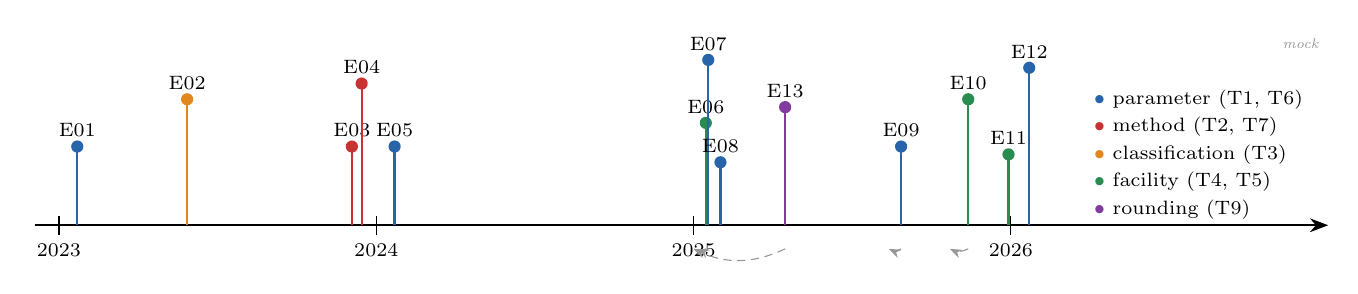
\begin{tikzpicture}[x=1.55cm]
\draw[-{Stealth}, thick] (0,0) -- (10.6,0);
\foreach \y/\x in {2023/0.2,2024/2.8,2025/5.4,2026/8.0}{\draw (\x,0.12)--(\x,-0.12) node[below,font=\scriptsize]{\y};}
\foreach \x/\lab/\c/\h in {0.35/E01/cdet/1, 1.25/E02/cai/1.6, 2.6/E03/cred/1, 2.68/E04/cred/1.8, 2.95/E05/cdet/1,
  5.5/E06/chum/1.3, 5.52/E07/cdet/2.1, 5.62/E08/cdet/0.8, 6.15/E13/cpur/1.5, 7.1/E09/cdet/1, 7.65/E10/chum/1.6, 7.98/E11/chum/0.9, 8.15/E12/cdet/2}{
  \draw[\c, thick] (\x,0) -- (\x,\h);
  \fill[\c] (\x,\h) circle (2.2pt) node[above, font=\scriptsize, text=black]{\lab};}
\foreach \a/\b in {5.5/5.4, 5.52/5.43, 7.1/7.0, 7.65/7.5, 6.15/5.4}{\draw[-{Stealth[length=1.5mm]}, cgr, densely dashed] (\a,-0.3) to[bend left=25] (\b,-0.3);}
\node[mock, anchor=east] at (10.6,2.3) {mock};
\node[font=\scriptsize, anchor=west] at (8.6,1.6) {\textcolor{cdet}{$\bullet$} parameter (T1, T6)};
\node[font=\scriptsize, anchor=west] at (8.6,1.25) {\textcolor{cred}{$\bullet$} method (T2, T7)};
\node[font=\scriptsize, anchor=west] at (8.6,0.9) {\textcolor{cai}{$\bullet$} classification (T3)};
\node[font=\scriptsize, anchor=west] at (8.6,0.55) {\textcolor{chum}{$\bullet$} facility (T4, T5)};
\node[font=\scriptsize, anchor=west] at (8.6,0.2) {\textcolor{cpur}{$\bullet$} rounding (T9)};
\end{tikzpicture}}
\caption{Regulation changes affecting Indonesian payroll income tax for permanent employees, 2023--2026. Markers show issue dates; arrows point back to the start of validity for retroactive rules.}
\label{fig:timeline}
\end{figure*}

\lipsum[94] % [pad]

\lipsum[5] \lipsum[6][1-6]

\lipsum[95] % [pad]

\lipsum[7][1-8] \cite{ref1,ref2,ref3}

\lipsum[96] % [pad]

\lipsum[8][1-3] \textbf{[Objective: the four properties under test, named as in Section~VII-A.]} \lipsum[8][4-6] Fig.~\ref{fig:arsitektur}. The contributions are as follows.
\begin{enumerate}
\item \lipsum[9][1-3]
\item \lipsum[10][1-3]
\item \lipsum[11][1-3]
\item \lipsum[12][1-2]
\end{enumerate}
\lipsum[13][1-2]

% ============================================================================
\lipsum[97] % [pad]

\section{Background: Payroll Income Tax in Indonesia}
% ============================================================================
\lipsum[14][1-3]

\lipsum[98] % [pad]

\subsection{Computing PPh~21 for a Permanent Employee}
\lipsum[15] Table~\ref{tab:slip} \lipsum[16][1-4]

\begin{table}[!t]
\caption{Running example: monthly PPh~21 of Employee A (status K/1, monthly salary Rp15\,000\,000, religious holiday allowance in March) under the annualised method (2023) and the effective-rate method (2024).}
\label{tab:slip}
\centering\scriptsize
\setlength{\tabcolsep}{4pt}
\begin{tabular}{@{}lrrcr@{}}
\toprule
Period & Gross (Rp) & 2023 (Rp) & TER 2024 & 2024 (Rp) \\
\midrule
January & 15\,xxx\,xxx & xxx\,xxx & B, x.x\% & xxx\,xxx \\
February & 15\,xxx\,xxx & xxx\,xxx & B, x.x\% & xxx\,xxx \\
March (THR) & 30\,xxx\,xxx & x\,xxx\,xxx & B, xx\% & x\,xxx\,xxx \\
April--November & 15\,xxx\,xxx & xxx\,xxx & B, x.x\% & xxx\,xxx \\
December & 15\,xxx\,xxx & xxx\,xxx & Art.~17 & xx\,xxx \\
\midrule
Year & xxx\,xxx\,xxx & x\,xxx\,xxx & & x\,xxx\,xxx \\
\bottomrule
\end{tabular}
\end{table}

\lipsum[99] % [pad]

\subsection{How Regulations Change}
\lipsum[17] Table~\ref{tab:jenis} \lipsum[18][1-3]

\begin{table}[!t]
\caption{Types of regulation change, with real examples.}
\label{tab:jenis}
\centering\scriptsize
\begin{tabularx}{\columnwidth}{@{}lLl@{}}
\toprule
Code & Type of change & Example \\
\midrule
T1 & Parameter value & E01 \\
T2 & Calculation method & E03 \\
T3 & Income classification & E02 \\
T4 & New facility & E06 \\
T5 & Facility scope extended & E10 \\
T6 & Validity extended & E09 \\
T7 & New table & E03 \\
T8 & Repeal without replacement & -- \\
T9 & Rounding rule & E13 \\
T10 & Company policy & collective labor agreements \\
\bottomrule
\end{tabularx}
\end{table}

\lipsum[100] % [pad]

\subsection{Company Policies and Their Legal Limits}
\lipsum[19] \lipsum[20][1-3]

\textbf{Scope and assumptions.}
\begin{itemize}
\item In scope: permanent employees of private and state-owned employers; one employee per computation; tax years 2023--2026 (development 2012--2022).
\item Out of scope: non-permanent workers, severance and other final-taxed income, the surcharge for employees without a tax identification number, batch payroll, withholding-slip reporting.
\item Assumptions: every employee has a valid tax identification; inputs are taken as recorded in payroll data.
\end{itemize}

% ============================================================================
\lipsum[101] % [pad]

\section{Related Work}
% ============================================================================
\lipsum[21][1-3]
\lipsum[102] % [pad]

\subsection{Rules as Code and Legal Knowledge-Based Systems}
\lipsum[22] \cite{ref4,ref5,ref6,ref7}
\lipsum[103] % [pad]

\subsection{Temporal Legal Knowledge Representation}
\lipsum[23] \cite{ref8,ref9,ref10}
\lipsum[104] % [pad]

\subsection{Incremental Knowledge Acquisition}
\lipsum[24][1-8] \cite{ref11,ref12}
\lipsum[105] % [pad]

\subsection{Large Language Models for Legal and Tax Formalization}
\lipsum[25] \lipsum[26][1-4] \cite{ref13,ref14,ref15,ref16,ref17}
\lipsum[106] % [pad]

\subsection{Evaluating Repeated LLM Updates}
\lipsum[27][1-8] \cite{ref18,ref19,ref20}
\lipsum[107] % [pad]

\subsection{Positioning}
\lipsum[28][1-5] Table~\ref{tab:posisi}.

\begin{table}[!t]
\caption{Positioning against the closest work.}
\label{tab:posisi}
\centering\scriptsize
\setlength{\tabcolsep}{2.5pt}
\begin{tabularx}{\columnwidth}{@{}LP{1.3cm}P{0.9cm}cccc@{}}
\toprule
Work & Representation & Author & Incr. & Prop. & Comp. & Exec. \\
\midrule
Catala & DSL & human & -- & -- & -- & \checkmark \\
Ripple-Down Rules & rules & expert & \checkmark & -- & -- & \checkmark \\
Veeramani et al. & graph & LLM & -- & -- & -- & \checkmark \\
Yadamsuren et al. & Prolog & LLM & -- & -- & -- & \checkmark \\
Lorenzo et al. & Catala & LLM & -- & -- & -- & -- \\
Jurayj et al. & Prolog & LLM & -- & -- & -- & \checkmark \\
Gogani-Khiabani et al. & Python & LLM & one step & -- & -- & \checkmark \\
Prior et al. & XML text & LLM & text & partly & -- & -- \\
\midrule
\textbf{This work} & graph + rules & LLM, gates & \checkmark & \checkmark & \checkmark & \checkmark \\
\bottomrule
\end{tabularx}
\end{table}

% ============================================================================
\lipsum[108] % [pad]

\section{Problem Formulation}
% ============================================================================
\lipsum[29][1-3]
\lipsum[109] % [pad]

\subsection{Knowledge Base and Computation Result}
\begin{definition}[Knowledge base]
\lipsum[30][1-3] A rule is a tuple $r = \langle \mathit{id}, \ell, \sigma, [t_s, t_e], t_c, \varphi, f \mathrel{:=} e, \mathit{src} \rangle$.
\end{definition}
\begin{definition}[Result]
\lipsum[31][1-2] We write $\mathit{result}(\mathcal{K}, x, t, \omega)$.
\end{definition}
\lipsum[32][1-4]

\lipsum[110] % [pad]

\subsection{Updates and Adaptivity Conditions}
\lipsum[33][1-3]
\begin{equation}
\mathit{result}(\mathcal{K}\oplus\hat{\Delta}, x, t, \omega) = \mathit{result}(\mathcal{K}^\star, x, t, \omega), \quad t \ge t_{\mathit{valid}},\ \omega \ge t_{\mathit{issued}}.
\end{equation}
\lipsum[34][1-5]

\lipsum[111] % [pad]

\subsection{Representational and Operational Adaptivity}
\lipsum[35][1-6]

\lipsum[112] % [pad]

\subsection{Error Types in a Chain of Updates}
\lipsum[36][1-6] Fig.~\ref{fig:galat}.

\begin{figure*}[!t]
\centering
\resizebox{0.95\textwidth}{!}{%
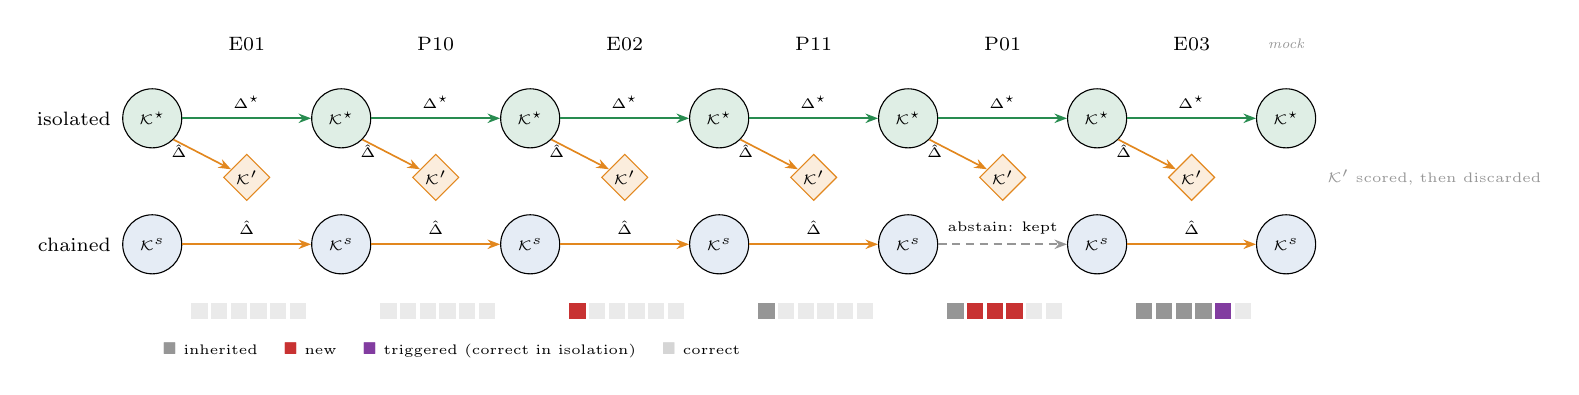
\begin{tikzpicture}[kb/.style={draw, circle, minimum size=0.75cm, font=\tiny, inner sep=0pt},
  sq/.style={minimum size=0.22cm, draw=white, line width=0.4pt, inner sep=0pt}]
\node[font=\scriptsize, anchor=east] at (-0.4,1.6) {isolated};
\node[font=\scriptsize, anchor=east] at (-0.4,0) {chained};
\foreach \e/\lab [count=\i from 0] in {E01/E01,P10/P10,E02/E02,P11/P11,P01/P01,E03/E03}{
  \node[font=\scriptsize] at (\i*2.4+1.2,2.55) {\lab};
  \node[kb, fill=chum!15] (g\i) at (\i*2.4,1.6) {$\mathcal{K}^\star$};
  \node[kb, fill=cdet!12] (c\i) at (\i*2.4,0) {$\mathcal{K}^{s}$};}
\node[kb, fill=chum!15] (g6) at (14.4,1.6) {$\mathcal{K}^\star$};
\node[kb, fill=cdet!12] (c6) at (14.4,0) {$\mathcal{K}^{s}$};
\foreach \i [evaluate=\i as \j using int(\i+1)] in {0,...,5}{
  \draw[ar, chum] (g\i) -- node[above, font=\tiny, text=black]{$\Delta^\star$} (g\j);
  \node[draw=cai, fill=cai!15, diamond, inner sep=1pt, font=\tiny] (k\i) at (\i*2.4+1.2,0.85) {$\mathcal{K}'$};
  \draw[ar, cai] (g\i.south east) -- node[left, font=\tiny, text=black, pos=0.4]{$\hat\Delta$} (k\i);}
\node[font=\tiny, text=cgr, anchor=west] at (14.8,0.85) {$\mathcal{K}'$ scored, then discarded};
\foreach \i [evaluate=\i as \j using int(\i+1)] in {0,1,2,3,5}{
  \draw[ar, cai] (c\i) -- node[above, font=\tiny, text=black]{$\hat\Delta$} (c\j);}
\draw[ar, cgr, densely dashed] (c4) -- node[above, font=\tiny, text=black]{abstain: kept} (c5);
\foreach \i/\cols in {0/{cgr!20,cgr!20,cgr!20,cgr!20,cgr!20,cgr!20}, 1/{cgr!20,cgr!20,cgr!20,cgr!20,cgr!20,cgr!20},
  2/{cred,cgr!20,cgr!20,cgr!20,cgr!20,cgr!20}, 3/{cgr,cgr!20,cgr!20,cgr!20,cgr!20,cgr!20},
  4/{cgr,cred,cred,cred,cgr!20,cgr!20}, 5/{cgr,cgr,cgr,cgr,cpur,cgr!20}}{
  \foreach \c [count=\k from 0] in \cols {\node[sq, fill=\c] at (\i*2.4+0.6+\k*0.25,-0.85) {};}}
\node[font=\tiny, anchor=west] at (0,-1.35) {\textcolor{cgr}{$\blacksquare$} inherited \quad \textcolor{cred}{$\blacksquare$} new \quad \textcolor{cpur}{$\blacksquare$} triggered (correct in isolation) \quad \textcolor{cgr!40}{$\blacksquare$} correct};
\node[mock] at (14.4,2.55) {mock};
\end{tikzpicture}}
\caption{Regulation replay protocol. Each event is applied in isolation to the gold knowledge base and in a chain to the system's own knowledge base; incorrect cases are inherited, new, or triggered by the chain.}
\label{fig:galat}
\end{figure*}

% ============================================================================
\lipsum[113] % [pad]

\section{Proposed System}
% ============================================================================
\lipsum[37][1-3]

\lipsum[114] % [pad]

\subsection{Architecture Overview}
\lipsum[38] Fig.~\ref{fig:arsitektur} \lipsum[39][1-3]

\begin{figure*}[!t]
\centering
\resizebox{0.95\textwidth}{!}{%
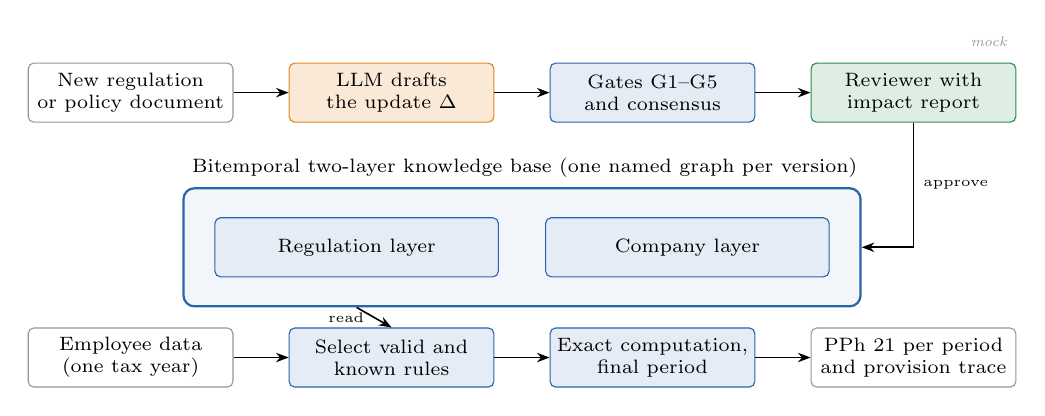
\begin{tikzpicture}[node distance=5mm and 7mm]
\node[bsrc, minimum width=2.6cm] (doc) {New regulation\\or policy document};
\node[bai, right=of doc, minimum width=2.6cm] (llm) {LLM drafts\\the update $\Delta$};
\node[bdet, right=of llm, minimum width=2.6cm] (gate) {Gates G1--G5\\and consensus};
\node[bhum, right=of gate, minimum width=2.6cm] (rev) {Reviewer with\\impact report};
\draw[ar] (doc)--(llm); \draw[ar] (llm)--(gate); \draw[ar] (gate)--(rev);
\node[draw=cdet, fill=cdet!6, thick, rounded corners, minimum width=8.6cm, minimum height=1.5cm, below=12mm of $(llm)!0.5!(gate)$] (kb) {};
\node[bdet, minimum width=3.6cm] at ($(kb.center)+(-2.1,0)$) {Regulation layer};
\node[bdet, minimum width=3.6cm] at ($(kb.center)+(2.1,0)$) {Company layer};
\node[font=\scriptsize, anchor=south west] at (kb.north west) {Bitemporal two-layer knowledge base (one named graph per version)};
\draw[ar] (rev.south) |- node[pos=0.25, right, font=\tiny]{approve} (kb.east);
\node[bsrc, below=26mm of doc, minimum width=2.6cm] (emp) {Employee data\\(one tax year)};
\node[bdet, right=of emp, minimum width=2.6cm] (sel) {Select valid and\\known rules};
\node[bdet, right=of sel, minimum width=2.6cm] (calc) {Exact computation,\\final period};
\node[bsrc, right=of calc, minimum width=2.6cm] (out) {PPh 21 per period\\and provision trace};
\draw[ar] (emp)--(sel); \draw[ar] (sel)--(calc); \draw[ar] (calc)--(out);
\draw[ar] (kb.south) ++(-2.1,0) -- node[left, font=\tiny]{read} (sel.north);
\node[mock, anchor=north east] at ($(rev.north east)+(0,0.45)$) {mock};
\end{tikzpicture}}
\caption{System architecture. The language model is used only to draft knowledge updates (top); every computation (bottom) is deterministic and traced to legal provisions.}
\label{fig:arsitektur}
\end{figure*}

\lipsum[115] % [pad]

\subsection{Knowledge Representation}
\lipsum[40] Fig.~\ref{fig:ontologi} \lipsum[41][1-5] Listing~\ref{lst:ter} \lipsum[42][1-3] Fig.~\ref{fig:bitemporal} \lipsum[43][1-4]

\begin{figure*}[!t]
\centering
\resizebox{0.9\textwidth}{!}{%
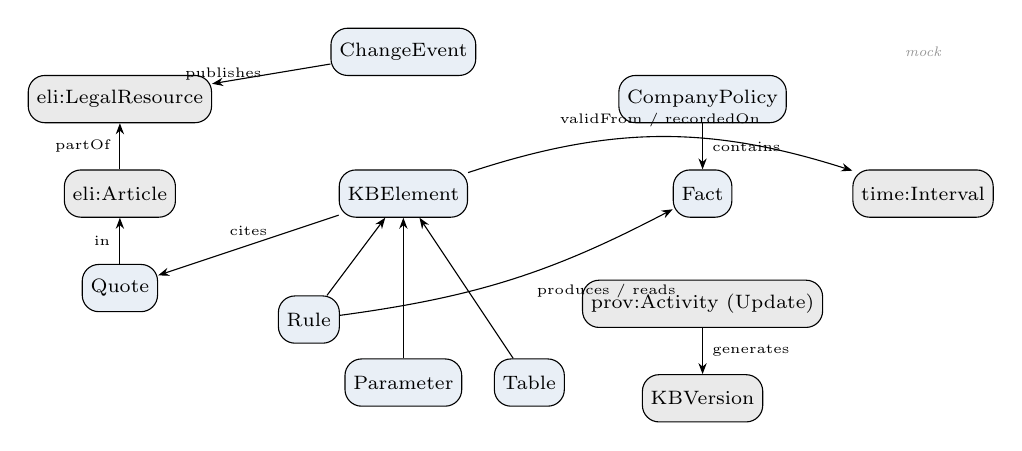
\begin{tikzpicture}[o/.style={draw, rounded corners=6pt, font=\scriptsize, fill=cdet!10, minimum height=0.6cm, inner sep=3pt},
  ox/.style={o, fill=cgr!20}, e/.style={-{Stealth[length=1.4mm]}, font=\tiny}]
\node[ox] (doc) at (0,2) {eli:LegalResource};
\node[ox] (art) at (0,0.8) {eli:Article};
\node[o] (quote) at (0,-0.4) {Quote};
\node[o] (el) at (3.6,0.8) {KBElement};
\node[o] (rule) at (2.4,-0.8) {Rule};
\node[o] (par) at (3.6,-1.6) {Parameter};
\node[o] (tab) at (5.2,-1.6) {Table};
\node[o] (fact) at (7.4,0.8) {Fact};
\node[o] (pol) at (7.4,2) {CompanyPolicy};
\node[o] (ev) at (3.6,2.6) {ChangeEvent};
\node[ox] (upd) at (7.4,-0.6) {prov:Activity (Update)};
\node[ox] (ver) at (7.4,-1.8) {KBVersion};
\node[ox] (time) at (10.2,0.8) {time:Interval};
\draw[e] (art)--node[left]{partOf}(doc); \draw[e] (quote)--node[left]{in}(art);
\draw[e] (el)--node[above]{cites}(quote); \draw[e] (rule)--(el); \draw[e] (par)--(el); \draw[e] (tab)--(el);
\draw[e] (rule) to[bend right=10] node[pos=0.55, below right]{produces / reads}(fact);
\draw[e] (pol)--node[right]{contains}(fact);
\draw[e] (ev)--node[left]{publishes}(doc);
\draw[e] (upd)--node[right]{generates}(ver);
\draw[e] (el) to[bend left=18] node[above, pos=0.5]{validFrom / recordedOn}(time);
\node[mock] at (10.2,2.6) {mock};
\end{tikzpicture}}
\caption{Ontology of the knowledge base. Reused vocabularies are shaded.}
\label{fig:ontologi}
\end{figure*}

\begin{listing}[!t]
\caption{The effective-rate withholding rule in Turtle (mock).}
\label{lst:ter}
\centering
\begin{minipage}{0.95\columnwidth}
\scriptsize
\begin{verbatim}
reg:REG.TER.RUNNING a pph:Rule ;
  pph:layer pph:Regulation ;
  pph:modality pph:Mandatory ;
  pph:produces fact:pph21_running ;
  pph:condition "not is_final_period" ;
  pph:expression "round(ter_rate * gross_income,
                  1, param('pph_round_mode'))" ;
  pph:validFrom "2024-01-01"^^xsd:date ;
  pph:recordedOn "2023-12-27"^^xsd:date ;
  pph:cites quote:PP-58-2023-P2-1 .
\end{verbatim}
\end{minipage}
\end{listing}

\begin{figure}[!t]
\centering
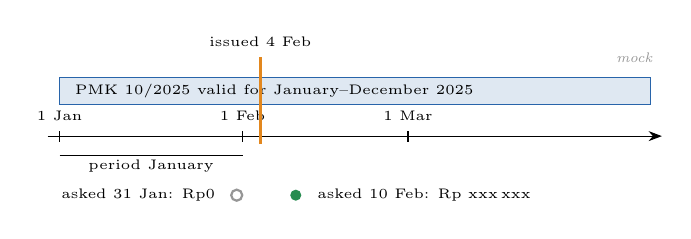
\begin{tikzpicture}[x=0.075cm]
\fill[cdet!15, draw=cdet] (0,1.0) rectangle (100,1.35);
\node[font=\tiny, anchor=west] at (1,1.175) {PMK 10/2025 valid for January--December 2025};
\draw[-{Stealth}] (-2,0.6) -- (102,0.6);
\foreach \x/\l in {0/1 Jan, 31/1 Feb, 59/1 Mar}{\draw (\x,0.53)--(\x,0.67) node[above, font=\tiny]{\l};}
\draw[cai, very thick] (34,0.5) -- (34,1.6) node[above, font=\tiny, text=black]{issued 4 Feb};
\draw[decorate] (0,0.35) -- (31,0.35); \node[font=\tiny] at (15.5,0.22) {period January};
\fill[white, draw=cgr, thick] (30,-0.15) circle (2pt); \node[font=\tiny, anchor=east] at (28,-0.15) {asked 31 Jan: Rp0};
\fill[chum] (40,-0.15) circle (2pt); \node[font=\tiny, anchor=west] at (42,-0.15) {asked 10 Feb: Rp xxx\,xxx};
\node[mock, anchor=east] at (102,1.6) {mock};
\end{tikzpicture}
\caption{Two time axes for Employee B. The same question about January 2025 gets the value that was correct with the knowledge of 31 January and the value that should have applied once PMK 10/2025 was issued.}
\label{fig:bitemporal}
\end{figure}

\lipsum[116] % [pad]

\subsection{Inference Engine}
\lipsum[44] Algorithm~\ref{alg:engine} \lipsum[45][1-4] Fig.~\ref{fig:engine}.

\begin{algorithm}[!t]
\caption{Inference engine for one case (mock)}
\label{alg:engine}
\footnotesize
\begin{algorithmic}[1]
\REQUIRE knowledge base $\mathcal{K}$, case $x$, knowledge date $\omega$
\FOR{each period $t$ of $x$}
  \FOR{each output fact $f$}
    \STATE $R \gets$ rules producing $f$, valid at $t$, recorded on or before $\omega$
    \STATE $R \gets \{r \in R : \varphi_r(x, t)\}$
    \STATE $r^* \gets$ winner of $R$ by rank, overrides, then recency
    \STATE evaluate $e_{r^*}$ on demand; record trace to provision
  \ENDFOR
\ENDFOR
\STATE recompute the year in the final period
\RETURN values, conflicts, trace
\end{algorithmic}
\end{algorithm}

\begin{figure*}[!t]
\centering
\resizebox{0.97\textwidth}{!}{%
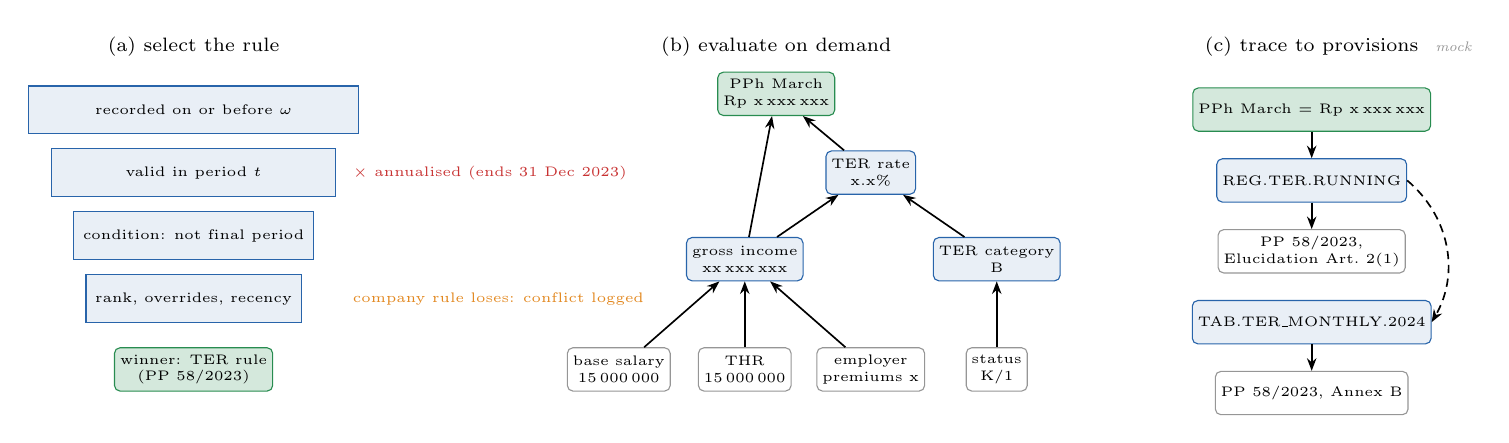
\begin{tikzpicture}[f/.style={draw=cdet, fill=cdet!10, rounded corners=2pt, font=\tiny, align=center, minimum height=0.55cm, inner sep=2pt},
  v/.style={font=\tiny\itshape, text=cdet}]
% (a) funnel
\node[font=\scriptsize] at (2.2,4.6) {(a) select the rule};
\foreach \y/\w/\t in {3.8/4.2/{recorded on or before $\omega$}, 3.0/3.6/{valid in period $t$}, 2.2/3.0/{condition: not final period}, 1.4/2.4/{rank, overrides, recency}}{
  \node[draw=cdet, fill=cdet!10, minimum width=\w cm, minimum height=0.6cm, font=\tiny] at (2.2,\y) {\t};}
\node[f, fill=chum!20, draw=chum] at (2.2,0.5) {winner: TER rule\\(PP 58/2023)};
\node[font=\tiny, text=cred, anchor=west] at (4.1,3.0) {$\times$ annualised (ends 31 Dec 2023)};
\node[font=\tiny, text=cai, anchor=west] at (4.1,1.4) {company rule loses: conflict logged};
% (b) dependency graph
\node[font=\scriptsize] at (9.6,4.6) {(b) evaluate on demand};
\node[f, fill=white, draw=cgr] (bs) at (7.6,0.5) {base salary\\15\,000\,000};
\node[f, fill=white, draw=cgr] (thr) at (9.2,0.5) {THR\\15\,000\,000};
\node[f, fill=white, draw=cgr] (prem) at (10.8,0.5) {employer\\premiums x};
\node[f, fill=white, draw=cgr] (st) at (12.4,0.5) {status\\K/1};
\node[f] (gross) at (9.2,1.9) {gross income\\xx\,xxx\,xxx};
\node[f] (cat) at (12.4,1.9) {TER category\\B};
\node[f] (rate) at (10.8,3.0) {TER rate\\x.x\%};
\node[f, fill=chum!20, draw=chum] (pph) at (9.6,4.0) {PPh March\\Rp x\,xxx\,xxx};
\draw[ar] (bs)--(gross); \draw[ar] (thr)--(gross); \draw[ar] (prem)--(gross); \draw[ar] (st)--(cat);
\draw[ar] (gross)--(rate); \draw[ar] (cat)--(rate); \draw[ar] (rate)--(pph); \draw[ar] (gross)--(pph);
% (c) trace
\node[font=\scriptsize] at (16.4,4.6) {(c) trace to provisions};
\node[f, fill=chum!20, draw=chum] (t1) at (16.4,3.8) {PPh March = Rp x\,xxx\,xxx};
\node[f] (t2) at (16.4,2.9) {REG.TER.RUNNING};
\node[f, fill=white, draw=cgr] (t3) at (16.4,2.0) {PP 58/2023,\\Elucidation Art.~2(1)};
\node[f] (t4) at (16.4,1.1) {TAB.TER\_MONTHLY.2024};
\node[f, fill=white, draw=cgr] (t5) at (16.4,0.2) {PP 58/2023, Annex B};
\draw[ar] (t1)--(t2); \draw[ar] (t2)--(t3); \draw[ar, densely dashed] (t2.east) to[bend left=40] (t4.east); \draw[ar] (t4)--(t5);
\node[mock] at (18.2,4.6) {mock};
\end{tikzpicture}}
\caption{How the inference engine computes one value: the withholding of Employee A for March 2024. (a) Rule selection, (b) on-demand evaluation of the fact dependency graph, (c) trace from the value to the legal provisions.}
\label{fig:engine}
\end{figure*}

\lipsum[117] % [pad]

\subsection{LLM-Assisted Knowledge Acquisition}
\lipsum[46] Fig.~\ref{fig:akuisisi} \lipsum[47] Table~\ref{tab:gerbang} \lipsum[48][1-5]

\begin{figure*}[!t]
\centering
\resizebox{0.95\textwidth}{!}{%
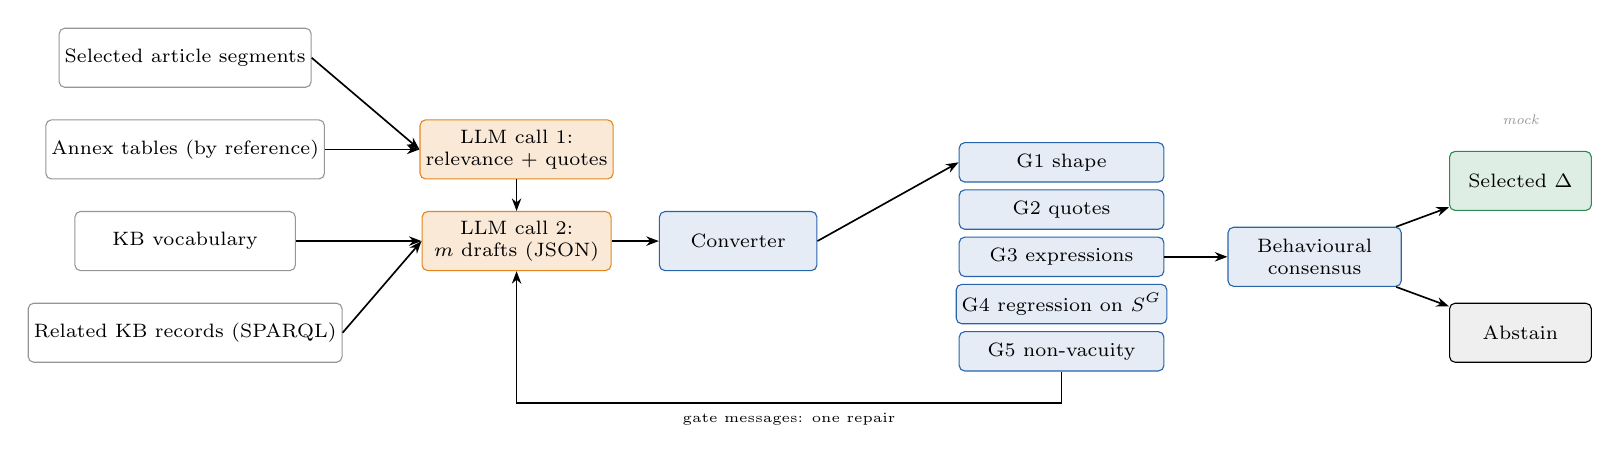
\begin{tikzpicture}[node distance=4mm and 6mm]
\node[bsrc, minimum width=2.8cm] (seg) {Selected article segments};
\node[bsrc, below=of seg, minimum width=2.8cm] (tab) {Annex tables (by reference)};
\node[bsrc, below=of tab, minimum width=2.8cm] (voc) {KB vocabulary};
\node[bsrc, below=of voc, minimum width=2.8cm] (rec) {Related KB records (SPARQL)};
\node[bai, right=12mm of tab, minimum width=2.4cm] (rel) {LLM call 1:\\relevance + quotes};
\node[bai, below=of rel, minimum width=2.4cm] (dr) {LLM call 2:\\$m$ drafts (JSON)};
\node[bdet, right=of dr, minimum width=2cm] (conv) {Converter};
\foreach \g/\n [count=\i] in {G1/shape,G2/quotes,G3/expressions,G4/regression on $S^G$,G5/non-vacuity}{
  \node[bdet, minimum width=2.6cm, minimum height=0.5cm] (g\i) at ($(conv.east)+(3.1,1.6-\i*0.6)$) {\g\ \n};}
\node[bdet, right=8mm of g3, minimum width=2.2cm] (cons) {Behavioural\\consensus};
\node[bhum, above right=2mm and 6mm of cons, minimum width=1.8cm] (sel) {Selected $\Delta$};
\node[b, below right=2mm and 6mm of cons, minimum width=1.8cm, fill=cgr!15] (abs) {Abstain};
\draw[ar] (seg.east) -- (rel.west); \draw[ar] (tab.east)--(rel.west); \draw[ar] (voc.east)--(dr.west); \draw[ar] (rec.east)--(dr.west);
\draw[ar] (rel)--(dr); \draw[ar] (dr)--(conv); \draw[ar] (conv.east)--(g1.west);
\draw[ar] (g5.south) -- ++(0,-0.4) -| node[pos=0.25, below, font=\tiny]{gate messages: one repair} (dr.south);
\draw[ar] (g3.east)--(cons); \draw[ar] (cons)--(sel); \draw[ar] (cons)--(abs);
\node[mock] at ($(sel.north)+(0,0.4)$) {mock};
\end{tikzpicture}}
\caption{Knowledge acquisition for one document. The model drafts; deterministic gates, behavioural consensus, and a human reviewer decide.}
\label{fig:akuisisi}
\end{figure*}

\begin{table}[!t]
\caption{Verification gates, what each checks, and failures observed in the experiments.}
\label{tab:gerbang}
\centering\scriptsize
\setlength{\tabcolsep}{3pt}
\begin{tabularx}{\columnwidth}{@{}lLLc@{}}
\toprule
Gate & Checks & Example failure & First fail \\
\midrule
G1 & schema, SHACL & lorem ipsum dolor & x \\
G2 & quotes, numbers, dates & sit amet consectetuer & x \\
G3 & expressions, dependencies & adipiscing elit & x \\
G4 & regression on $S^G$ & engine error on $\mathcal{K}'$ & x \\
G5 & non-vacuity & element changes nothing & x \\
\midrule
\multicolumn{3}{@{}l}{Initial drafts rejected} & xx/49 \\
\bottomrule
\end{tabularx}
\end{table}

\lipsum[118] % [pad]

\subsection{Cross-Layer Impact Analysis}
\lipsum[49][1-7]

\lipsum[119] % [pad]

\subsection{Application and Human Review Workflow}
\lipsum[50] Fig.~\ref{fig:layar}.

\begin{figure*}[!t]
\centering
\resizebox{0.95\textwidth}{!}{%
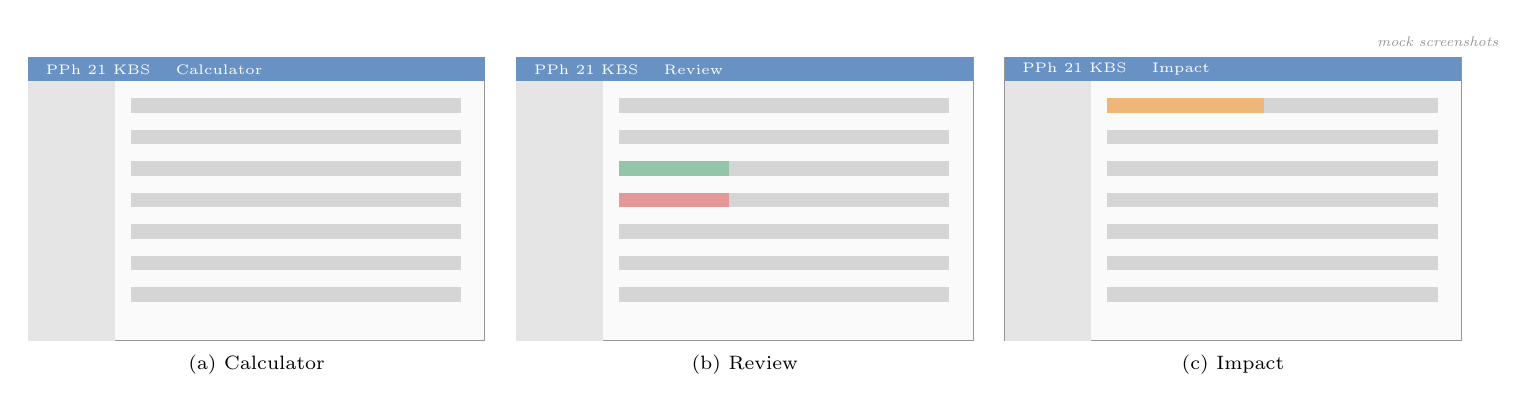
\begin{tikzpicture}
\foreach \px/\lab/\t in {0/(a)/Calculator, 6.2/(b)/Review, 12.4/(c)/Impact}{
  \draw[cgr, fill=cgr!5] (\px,0) rectangle ++(5.8,3.6);
  \fill[cdet!70] (\px,3.3) rectangle ++(5.8,0.3);
  \node[font=\tiny, text=white, anchor=west] at (\px+0.1,3.45) {PPh 21 KBS \quad \t};
  \fill[cgr!25] (\px,0) rectangle ++(1.1,3.3);
  \foreach \y in {2.9,2.5,2.1,1.7,1.3,0.9,0.5}{\fill[cgr!40] (\px+1.3,\y) rectangle ++(4.2,0.18);}
  \node[font=\scriptsize] at (\px+2.9,-0.3) {\lab\ \t};}
\fill[chum!50] (7.5,2.1) rectangle ++(1.4,0.18); \fill[cred!50] (7.5,1.7) rectangle ++(1.4,0.18);
\fill[cai!60] (13.7,2.9) rectangle ++(2,0.18);
\node[mock] at (17.9,3.8) {mock screenshots};
\end{tikzpicture}}
\caption{The application: (a) calculator with provision trace, (b) review of a drafted update with before/after results, (c) impact report on company policies.}
\label{fig:layar}
\end{figure*}

% ============================================================================
\lipsum[120] % [pad]

\section{Case Study: Adapting to the Effective-Rate Method}
% ============================================================================
\lipsum[51] Fig.~\ref{fig:kasus} \lipsum[52] \lipsum[53][1-5]

\begin{figure*}[!t]
\centering
\resizebox{0.95\textwidth}{!}{%
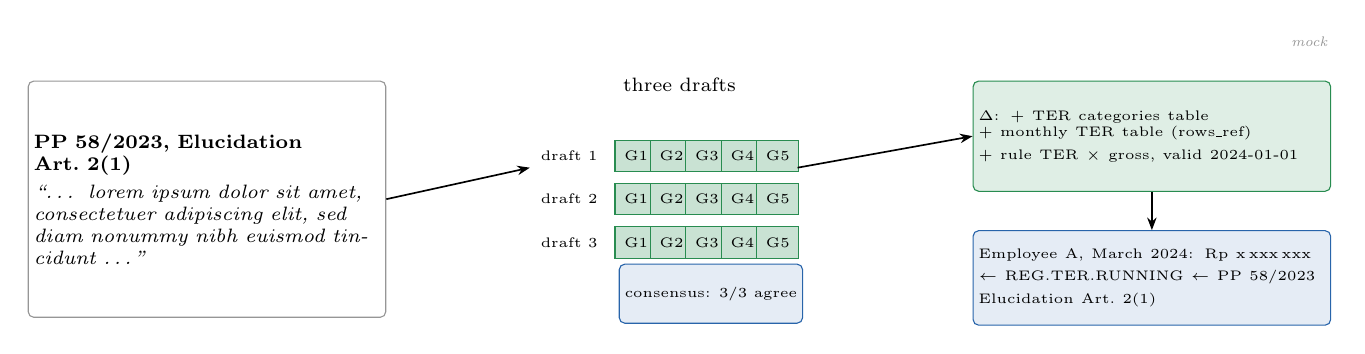
\begin{tikzpicture}
\node[bsrc, text width=4.4cm, align=left, minimum height=3cm] (q) at (0,0) {\textbf{PP 58/2023, Elucidation Art.~2(1)}\\[2pt]\itshape ``\ldots{} lorem ipsum dolor sit amet, consectetuer adipiscing elit, sed diam nonummy nibh euismod tincidunt \ldots''};
\node[font=\scriptsize] at (6,1.45) {three drafts};
\foreach \d [count=\i] in {1,2,3}{
  \node[font=\tiny] at (4.6,1.1-\i*0.55) {draft \d};
  \foreach \g [count=\j] in {G1,G2,G3,G4,G5}{\node[draw=chum, fill=chum!25, font=\tiny, minimum size=0.4cm] at (5+\j*0.45,1.1-\i*0.55) {\g};}}
\node[bdet, font=\tiny] at (6.4,-1.2) {consensus: 3/3 agree};
\node[bhum, text width=4.4cm, align=left, minimum height=1.4cm] (d) at (12,0.8) {\tiny $\Delta$: + TER categories table\\+ monthly TER table (rows\_ref)\\+ rule TER $\times$ gross, valid 2024-01-01};
\node[bdet, text width=4.4cm, align=left, minimum height=1.2cm] (t) at (12,-1) {\tiny Employee A, March 2024: Rp x\,xxx\,xxx\\$\leftarrow$ REG.TER.RUNNING $\leftarrow$ PP 58/2023 Elucidation Art.~2(1)};
\draw[ar] (q.east)--(4.1,0.4); \draw[ar] (7.5,0.4)--(d.west); \draw[ar] (d)--(t);
\node[mock] at (14,2) {mock};
\end{tikzpicture}}
\caption{Case study: from the text of PP 58/2023 to an approved knowledge update and a traced withholding value for Employee A.}
\label{fig:kasus}
\end{figure*}

% ============================================================================
\lipsum[121] % [pad]

\section{Evaluation Design}
% ============================================================================
\lipsum[122] % [pad]

\subsection{Properties under Test}
\lipsum[54][1-8] Table~\ref{tab:petaeval}.

\begin{table*}[!t]
\caption{Evaluation map: properties, experiments, data, metrics, and preregistered hypotheses.}
\label{tab:petaeval}
\centering\scriptsize
\begin{tabularx}{\textwidth}{@{}P{3.0cm}P{0.8cm}P{3.2cm}LP{3.2cm}P{1.3cm}@{}}
\toprule
Property & Exp. & Data & Metric (one-line definition) & Hypothesis & Status \\
\midrule
Instrument validity & E0 & four references, mutants & exact agreement; mutation score & -- & registered \\
Expressiveness & E1 & 16 unseen changes & representational adaptability: lorem ipsum dolor & H1: lower bound $\ge$ 0.70 & registered \\
Safety of one update & E2 & 18 real documents, 20 distractors & correct, silent error, abstain: lorem ipsum dolor sit amet & H2a, H2b & registered \\
Stability of chained updates & E3 & 33 events, 150 cases/year & stability; triggered errors; final-chain errors & H3a, H3b & registered / expl. \\
Impact detection & E4 & 134 policy--event pairs & recall, precision, $F_2$ & H4a, H4b & registered \\
Comparison & E5 & code history; 100 cases & days, lines; exact match & -- & exploratory \\
\bottomrule
\end{tabularx}
\end{table*}

\lipsum[123] % [pad]

\subsection{Regulation Replay Protocol}
\lipsum[55] \lipsum[56][1-4]

\lipsum[124] % [pad]

\subsection{Data and Temporal Split}
\lipsum[57][1-7] Table~\ref{tab:korpus} in Appendix~D.
\lipsum[125] % [pad]

\subsection{Ground Truth and Instrument Validation}
\lipsum[58] \lipsum[59][1-4]

\lipsum[126] % [pad]

\subsection{Test Space and Coverage}
\lipsum[60][1-6] Fig.~\ref{fig:cakupan}.

\begin{figure}[!t]
\centering
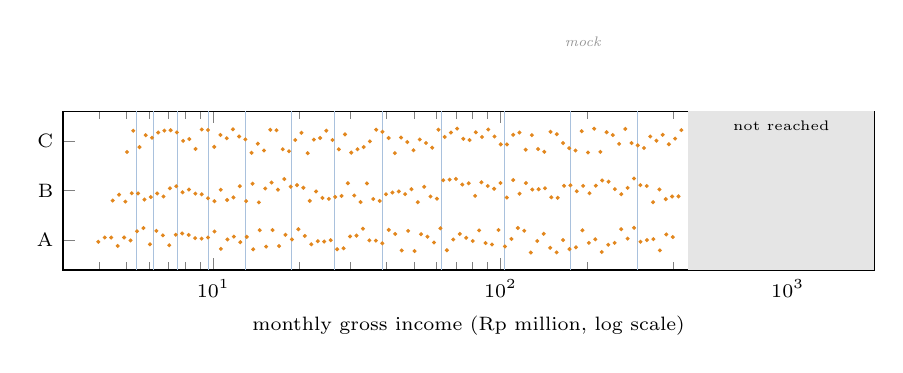
\begin{tikzpicture}
\pgfmathsetseed{7}
\begin{axis}[width=0.98\columnwidth, height=3.6cm, xmode=log, xmin=3, xmax=2000, ymin=0.4, ymax=3.6,
  ytick={1,2,3}, yticklabels={A,B,C}, xlabel={monthly gross income (Rp million, log scale)},
  tick label style={font=\scriptsize}, label style={font=\scriptsize}]
\fill[cgr!25] (axis cs:450,0.4) rectangle (axis cs:2000,3.6);
\node[font=\tiny] at (axis cs:950,3.3) {not reached};
\pgfplotsinvokeforeach{5.4,6.2,7.5,9.65,12.95,18.75,26.45,38.9,62.2,103,175,300}{\draw[cdet!40] (axis cs:#1,0.4) -- (axis cs:#1,3.6);}
\addplot[only marks, mark size=0.5pt, cai, samples=90, domain=0.6:2.6] ({10^x}, {1+0.25*rand});
\addplot[only marks, mark size=0.5pt, cai, samples=90, domain=0.65:2.62] ({10^x}, {2+0.25*rand});
\addplot[only marks, mark size=0.5pt, cai, samples=90, domain=0.7:2.63] ({10^x}, {3+0.25*rand});
\end{axis}
\node[mock] at (6.6,2.9) {mock};
\end{tikzpicture}
\caption{Coverage of the test space: test cases against the effective-rate brackets (lines). The shaded range is not reached.}
\label{fig:cakupan}
\end{figure}

\lipsum[127] % [pad]

\subsection{Metrics}
\lipsum[61] \lipsum[62][1-5]
\begin{equation}
\mathrm{SER} = \frac{1}{|D|}\sum_{d\in D} \mathbf{1}[\text{wrong}_d], \qquad \mathrm{CAR} = \frac{1}{|D|}\sum_{d\in D} \mathbf{1}[\text{correct}_d].
\end{equation}
\lipsum[63][1-4]

\lipsum[128] % [pad]

\subsection{Baselines and Ablations}
\lipsum[64][1-8]

\lipsum[129] % [pad]

\subsection{Statistical Analysis and Preregistration}
\lipsum[65][1-7]

\lipsum[130] % [pad]

\subsection{Implementation and Cost}
\lipsum[66][1-5]

% ============================================================================
\lipsum[131] % [pad]

\section{Results}
% ============================================================================
\lipsum[67][1-3] Table~\ref{tab:putusan}.

\begin{table*}[!t]
\caption{Hypotheses and verdicts. Exploratory analyses are marked.}
\label{tab:putusan}
\centering\scriptsize
\begin{tabularx}{\textwidth}{@{}P{5.2cm}LP{3.6cm}@{}}
\toprule
Hypothesis & Result & Verdict \\
\midrule
Invariants A1 and A3$_\omega$ & lorem ipsum & \xx \\
H1: lower bound of RA $\ge 0.70$ & lorem ipsum dolor sit amet (x.xxx) & \xx \\
H2a: upper bound of SER $\le 0.25$ & lorem ipsum (x.xxx) & \xx \\
H2b: CAR above B3 and B4 & lorem ipsum dolor & \xx \\
H2b: non-inferiority of SER & lorem ipsum dolor sit & \xx \\
H3a: lower bound of OAR $\ge 0.75$ & lorem ipsum & \xx \\
H3b: triggered errors within noise & lorem ipsum & \xx \\
H4a: lower bound of recall $\ge 0.70$ & lorem ipsum & \xx \\
H4b: $F_2$ above simple detectors & lorem ipsum & \xx \\
\bottomrule
\end{tabularx}
\end{table*}

\lipsum[132] % [pad]

\subsection{Instrument Validity}
\lipsum[68] Table~\ref{tab:acuan} in Appendix~D.
\lipsum[133] % [pad]

\subsection{Expressiveness of the Representation}
\lipsum[69][1-8] Table~\ref{tab:unseen} in Appendix~D.

\lipsum[134] % [pad]

\subsection{Single-Document Acquisition}
\lipsum[70] Fig.~\ref{fig:ukuran}. \lipsum[71][1-6]
\begin{figure*}[!t]
\centering
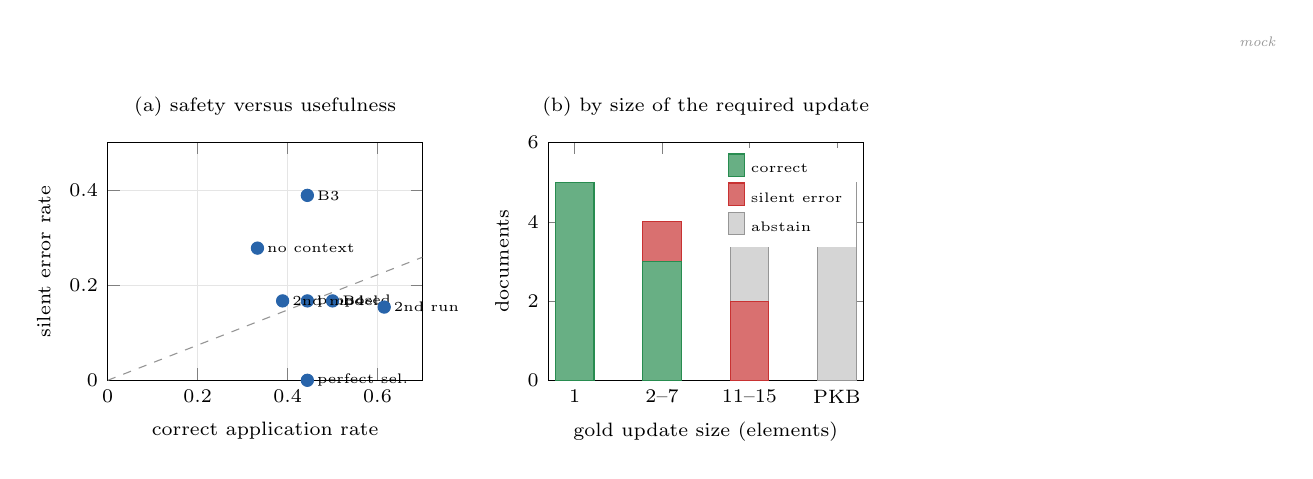
\begin{tikzpicture}
\begin{groupplot}[group style={group size=2 by 1, horizontal sep=1.6cm}, width=0.46\textwidth, height=4.6cm,
  tick label style={font=\scriptsize}, label style={font=\scriptsize}, title style={font=\scriptsize}]
\nextgroupplot[title={(a) safety versus usefulness}, xmin=0, xmax=0.7, ymin=0, ymax=0.5,
  xlabel={correct application rate}, ylabel={silent error rate}, grid=major, grid style={cgr!25}]
\addplot[only marks, mark=*, mark size=2.2pt, cdet, nodes near coords, point meta=explicit symbolic,
  every node near coord/.style={font=\tiny, anchor=west, text=black}] coordinates {
  (0.444,0.167) [proposed] (0.615,0.154) [2nd run] (0.444,0.389) [B3] (0.5,0.167) [B4]
  (0.333,0.278) [no context] (0.389,0.167) [2nd model] (0.444,0.0) [perfect sel.]};
\addplot[cgr, dashed, domain=0:0.7] {0.27/0.73*x};
\nextgroupplot[title={(b) by size of the required update}, ybar stacked, bar width=14pt, ymin=0, ymax=6,
  symbolic x coords={1,2--7,11--15,PKB}, xtick=data, xlabel={gold update size (elements)}, ylabel={documents},
  legend style={font=\tiny, at={(0.98,0.98)}, anchor=north east, draw=none}, legend cell align=left]
\addplot[fill=chum!70, draw=chum] coordinates {(1,5) (2--7,3) (11--15,0) (PKB,0)};
\addplot[fill=cred!70, draw=cred] coordinates {(1,0) (2--7,1) (11--15,2) (PKB,0)};
\addplot[fill=cgr!40, draw=cgr] coordinates {(1,0) (2--7,0) (11--15,2) (PKB,5)};
\legend{correct, silent error, abstain}
\end{groupplot}
\node[mock] at (14.6,4.3) {mock};
\end{tikzpicture}
\caption{Single-document acquisition on 18 real documents (13 regulations, 5 collective labor agreements): (a) safety versus usefulness by condition, (b) outcome by the size of the required update.}
\label{fig:ukuran}
\end{figure*}

\lipsum[135] % [pad]

\subsection{Component Ablation}
\lipsum[72] Table~\ref{tab:ablasi}.

\begin{table}[!t]
\caption{Ablation of pipeline components.}
\label{tab:ablasi}
\centering\scriptsize
\setlength{\tabcolsep}{2.5pt}
\begin{tabularx}{\columnwidth}{@{}LP{2.2cm}cccc@{}}
\toprule
Condition & Question & C & S & A & Broken \\
\midrule
Full pipeline & -- & x & x & x & x \\
No KB context & lorem ipsum & x & x & x & x \\
No G2 & dolor sit amet & x & x & x & x \\
No G3 & consectetuer & x & x & x & x \\
No G4 & adipiscing & x & x & x & x \\
No G5 & elit sed & x & x & x & x \\
G1 only & diam nonummy & x & x & x & x \\
No repair & nibh euismod & x & x & x & x \\
First draft & tincidunt ut & x & x & x & x \\
Perfect selection & laoreet & x & x & x & x \\
\bottomrule
\multicolumn{6}{@{}p{\columnwidth}@{}}{\tiny C correct, S silent error, A abstain. Notes: from-scratch formalisation lorem ipsum; SHACL rejected x of xxx drafts.}
\end{tabularx}
\end{table}

\lipsum[136] % [pad]

\subsection{Chained Replay, 2023--2026}
\lipsum[73] Fig.~\ref{fig:replay} \lipsum[74][1-5]

\begin{figure*}[!t]
\centering
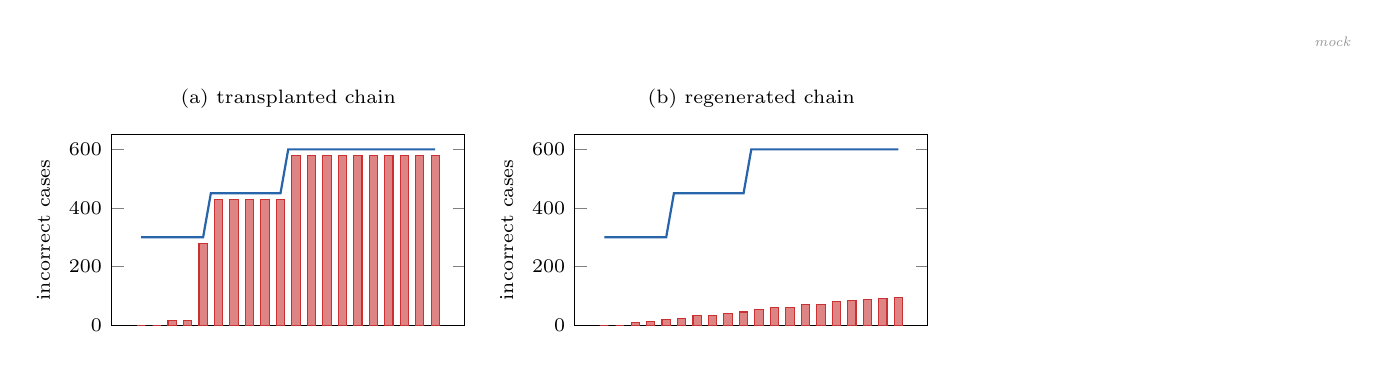
\begin{tikzpicture}
\begin{groupplot}[group style={group size=2 by 1, horizontal sep=1.4cm}, ybar, width=0.5\textwidth, height=4cm, ymin=0, ymax=650, /pgf/bar width=3pt,
  xtick=\empty, ylabel={incorrect cases}, tick label style={font=\scriptsize}, label style={font=\scriptsize}, title style={font=\scriptsize}]
\nextgroupplot[title={(a) transplanted chain}]
\addplot[fill=cred!60, draw=cred] coordinates {(1,0)(2,0)(3,15)(4,15)(5,279)(6,429)(7,429)(8,429)(9,429)(10,429)(11,579)(12,579)(13,579)(14,579)(15,579)(16,579)(17,579)(18,579)(19,579)(20,579)};
\addplot[sharp plot, cdet, thick, bar shift=0pt] coordinates {(1,300)(5,300)(5.5,450)(10,450)(10.5,600)(20,600)};
\nextgroupplot[title={(b) regenerated chain}]
\addplot[fill=cred!60, draw=cred] coordinates {(1,0)(2,0)(3,10)(4,12)(5,20)(6,24)(7,32)(8,32)(9,40)(10,45)(11,52)(12,60)(13,61)(14,70)(15,72)(16,80)(17,85)(18,88)(19,90)(20,93)};
\addplot[sharp plot, cdet, thick, bar shift=0pt] coordinates {(1,300)(5,300)(5.5,450)(10,450)(10.5,600)(20,600)};
\end{groupplot}
\node[mock] at (15.5,3.6) {mock};
\end{tikzpicture}
\caption{Regulation replay. Bars show incorrect employee-year cases after each event; the line shows the number of cases evaluated.}
\label{fig:replay}
\end{figure*}

\lipsum[137] % [pad]

\subsection{Cross-Layer Impact Detection}
\lipsum[75][1-8]

\lipsum[138] % [pad]

\subsection{Comparison with Code Maintenance and Direct LLM Calculation}
\lipsum[76] Fig.~\ref{fig:adaptasi}. Table~\ref{tab:b2} in Appendix~D.

\begin{figure}[!t]
\centering
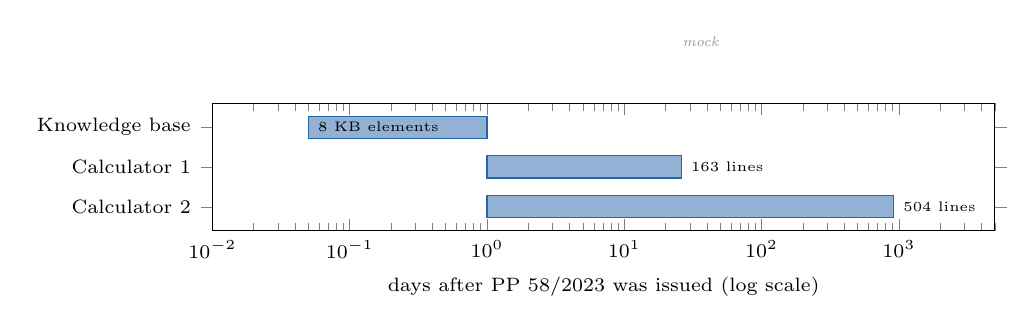
\begin{tikzpicture}
\begin{axis}[xbar, width=0.95\columnwidth, height=3.2cm, xmode=log, xmin=0.01, xmax=5000, bar width=8pt,
  symbolic y coords={Calculator 2,Calculator 1,Knowledge base}, ytick=data, xlabel={days after PP 58/2023 was issued (log scale)},
  nodes near coords, nodes near coords style={font=\tiny, anchor=west}, point meta=explicit symbolic,
  tick label style={font=\scriptsize}, label style={font=\scriptsize}, enlarge y limits=0.3]
\addplot[fill=cdet!50, draw=cdet] coordinates {(0.05,Knowledge base) [8 KB elements] (26,Calculator 1) [163 lines] (915,Calculator 2) [504 lines]};
\end{axis}
\node[mock] at (6.2,2.4) {mock};
\end{tikzpicture}
\caption{Time to adapt to the effective-rate method after PP 58/2023 was issued: the knowledge base versus two open-source calculators, with the size of each change.}
\label{fig:adaptasi}
\end{figure}
% ============================================================================
\lipsum[139] % [pad]

\section{Discussion}
% ============================================================================
\lipsum[140] % [pad]

\subsection{When Can LLM-Drafted Updates Be Trusted?}
\lipsum[77][1-8]
\lipsum[141] % [pad]

\subsection{Why LLM Updates Fail}
\lipsum[78] Table~\ref{tab:taksonomi}. \lipsum[79][1-5]

\begin{table}[!t]
\caption{Error taxonomy of drafted updates.}
\label{tab:taksonomi}
\centering\scriptsize
\begin{tabularx}{\columnwidth}{@{}Lccl@{}}
\toprule
Category & Drafts & Documents & Example \\
\midrule
Wrong scope & x & x & E02, E11 \\
Missed exception & x & x & lorem \\
Case-attribute name & x & x & E07 \\
Distractor applied & x & x & P01 \\
Incomplete update & x & x & ipsum \\
Malformed, caught by gates & xx & xx & G1--G5 \\
\bottomrule
\end{tabularx}
\end{table}
\lipsum[142] % [pad]

\subsection{Implications for Payroll Practice}
\lipsum[80][1-7] \textbf{[Operational limits: when a draft must not be applied without full review.]}
\lipsum[143] % [pad]

\subsection{Implications for Knowledge-Based Systems and Legal AI}
\lipsum[81][1-6] The following design recommendations follow from the results.
\begin{enumerate}
\item Require a verbatim quote for every number and date.
\item Draw several drafts and allow abstention.
\item Route every abstention to a reviewer queue.
\item Check scope completeness and case-attribute names.
\item Evaluate by chronological replay, not on a single legal state.
\end{enumerate}
\lipsum[144] % [pad]

\subsection{Threats to Validity}
\lipsum[82] \lipsum[83][1-6]
\lipsum[145] % [pad]

\subsection{Limitations}
\lipsum[84][1-6]

% ============================================================================
\lipsum[146] % [pad]

\section{Conclusion}
% ============================================================================
\lipsum[85][1-8]

\lipsum[147] % [pad]

\section*{Data and Code Availability}
\lipsum[86][1-4]

\appendices
\section{Notation and Glossary}
\lipsum[87][1-6]
\section{Taxonomies}
\lipsum[88][1-6]
\section{Gate Specification and Acquisition Algorithm}
\lipsum[89][1-8]

\section{Test Corpus and Additional Results}
\lipsum[95][1-3]

\begin{table}[!t]
\caption{Test corpus.}
\label{tab:korpus}
\centering\scriptsize
\setlength{\tabcolsep}{3pt}
\begin{tabularx}{\columnwidth}{@{}lLlc@{}}
\toprule
ID & Document & Type & $|\Delta^\star|$ \\
\midrule
E01 & Pension wage cap 2023 & T1 & 1 \\
E02 & PMK 66/2023 (benefits in kind) & T3 & 15 \\
E03 & PP 58/2023 (TER) & T2, T7 & 7 \\
\multicolumn{4}{@{}c}{\textcolor{cgr}{\ldots}} \\
E13 & PER-11/PJ/2025 (rounding) & T9 & 1 \\
\midrule
P01--P20 & 20 distractors & -- & 0 \\
-- & 5 collective labor agreements & T10 & 14--35 \\
-- & 14 synthetic policies & T10 & 1--7 \\
-- & 4 counterfactuals & T1, T3, T4 & -- \\
U01--U16 & 16 unseen changes & various & -- \\
\bottomrule
\end{tabularx}
\end{table}

\begin{table}[!t]
\caption{Agreement of the knowledge base and engine with external references.}
\label{tab:acuan}
\centering\scriptsize
\setlength{\tabcolsep}{3pt}
\begin{tabularx}{\columnwidth}{@{}lccccL@{}}
\toprule
Reference & Cases & Obs. & $\le$Rp1 & Material & Note \\
\midrule
GT1 development & \nn & \nn & \nn & \nn & lorem \\
GT1 holdout & \nn & \nn & \nn & \nn & ipsum \\
GT2 DJP calculator & \nn & \nn & \nn & \nn & dolor \\
GT3 independent & \nn & \nn & \nn & \nn & sit \\
GT5 policy examples & -- & \nn & \nn & \nn & amet \\
\bottomrule
\end{tabularx}
\end{table}

\begin{table}[!t]
\caption{Engine versus direct LLM calculation by case complexity.}
\label{tab:b2}
\centering\scriptsize
\setlength{\tabcolsep}{3pt}
\begin{tabularx}{\columnwidth}{@{}Lccccc@{}}
\toprule
Complexity & $n$ & Engine & LLM exact & LLM $\le$Rp1 & Material \\
\midrule
Fixed salary only & xx & xx & xx & xx & xx \\
With THR or bonus & xx & xx & xx & xx & xx \\
Benefits in kind & xx & xx & xx & xx & xx \\
Gross-up & xx & xx & xx & xx & xx \\
Government-borne tax & xx & xx & xx & xx & xx \\
Mid-year entry or exit & xx & xx & xx & xx & xx \\
\bottomrule
\end{tabularx}
\end{table}

\begin{table}[!t]
\caption{The 16 unseen changes and whether they could be expressed without changing the engine.}
\label{tab:unseen}
\centering\scriptsize
\setlength{\tabcolsep}{3pt}
\begin{tabularx}{\columnwidth}{@{}lLcccc@{}}
\toprule
ID & Type of change & Ex. & Aligned & Not aligned & Max diff \\
\midrule
U01 & lorem ipsum & x & \checkmark & \checkmark & 0 \\
U02 & dolor sit & x & \checkmark & -- & x \\
\multicolumn{6}{@{}c}{\textcolor{cgr}{\ldots}} \\
U16 & amet & x & \checkmark & \checkmark & 0 \\
\midrule
Total & & 100 & 16/16 & 8/16 & xx \\
\bottomrule
\end{tabularx}
\end{table}

\section*{Acknowledgment}
\lipsum[90][1-4]

% ---------------------------------------------------------------- rujukan tiruan
\begin{thebibliography}{48}
\newcount\rc \rc=0
\loop\advance\rc by 1
\edef\rkey{ref\the\rc}
\expandafter\bibitem\expandafter{\rkey} A. Author and B. Author, ``Lorem ipsum dolor sit amet, consectetuer adipiscing elit,'' \textit{Journal of Lorem Ipsum}, vol.~\the\rc, no.~2, pp.~1--10, 2024, doi: 10.0000/mock.\the\rc.
\ifnum\rc<48\repeat
\end{thebibliography}

\begin{IEEEbiography}[{
\includegraphics[width=1in,height=1.25in,clip,keepaspectratio]{author1.png}}]{Obi Kastanya}
\lipsum[91][1-5]
\end{IEEEbiography}

\begin{IEEEbiography}[{
\includegraphics[width=1in,height=1.25in,clip,keepaspectratio]{author2.png}}]{Mahathir Muhammad}
\lipsum[92][1-5]
\end{IEEEbiography}

\EOD
\end{document}
